\documentclass{report}[12pt]

\usepackage{mathtools,enumitem,amssymb,amsmath,kotex,amsfonts,listings,stmaryrd,amsthm}
\usepackage{xfrac,txfonts}
\usepackage{graphicx}
\usepackage{mathrsfs}
\usepackage{subcaption}
\usepackage{ebproof}
\usepackage{tikz}
\usepackage{xcolor}
\usepackage[stable]{footmisc} % This package allows to use footnote in section.

\usetikzlibrary{trees}
\usetikzlibrary{cd}
\usetikzlibrary{arrows,decorations.pathmorphing,backgrounds,positioning,fit,petri,bending}
\begin{document}

\setlength\parindent{0pt}

\newtheoremstyle{break}
  {\topsep}{\topsep}%
  {\itshape}{}%
  {\bfseries}{}%
  {\newline}{}%

\theoremstyle{break}

\newtheorem{theorem}{Theorem}[section]
\newtheorem{definition}{Definition}
\newtheorem{proposition}{Proposition}
\newtheorem{corollary}{Corollary}
\newtheorem{lemma}{Lemma}
\newtheorem{example}{Example}
\newcommand{\nonterminal}[1]{\langle \text{#1}\rangle}
\newcommand{\rem}[0]{\text{ rem }}
\newcommand{\interp}[1]{\llbracket #1 \rrbracket}
\newcommand{\bbot}[0]{\Perp}
\newcommand{\TODO}[1]{TODO : #1}

\setcounter{chapter}{8}

\title{CS520 Lecture 8\\Recursively Defined Domains}
\maketitle

\section{Motivation}
1. One reason that we studied category thoery is to understand a general principle behind the construction of recursively defined domains, such as the following $\Omega$ that you encountered before:
\begin{align*}
  &\Omega \backsimeq (\hat \Sigma + \mathbb{Z}\times \Omega + (\mathbb{Z}\rightarrow \Omega))_\bot \\
  & \hat \Sigma \stackrel{def}{=} \Sigma \cup \{abort\}\times \Sigma (\backsimeq \Sigma + \Sigma)
\end{align*}
2. If we write the RHS of the above isomorphism as $F(\Omega)$, the formula says: $\Omega \backsimeq F(\Omega)$ that is, $\Omega$ is a fixed point of $F$. In fact, $\Omega$ is not just a fixed point, but the best fixed point. where "the best" means something very similar to "the least" in the standard fixed point theorem of the domain theory.

3. We will generalize the standard least fixed point theorem of the domain theory and obtain a general categorical least fixed point theorem. This generalization closely follows the intuition that categories are generalized partially ordered sets (and functors are generalized monotone functions). Then, we will instantiate our generalization with a particular category constructed out of domains and a particular kind of continuous functions called embeddings.

\section{$\omega$\footnote{omega, meaning the first countable ordinal}-chain and Co-limit of $\omega$-chain}
1. Let's start by  remembering ingredients that we needed when expressing the standard least fixed point theorem of the domain theory.
\begin{itemize}
  \item A partially ordered set $D$ has the least element.
  \item Every chain in $D$ has the least upper bound.
  \item A function $f$ on $D$ is continuous. (i.e., monotone and chain-limit-preserving)
\end{itemize}
Then, the theorem says that $f$ has the least fixed point $x_0$. That is, $f(x_0) = x_0$ and for all $y$ s.t. $f(y) \sqsubseteq y$, $x_0 \sqsubseteq y$\footnote{property that is a bit stronger than $x_0$ being the least fixed point}.

2. In the categorical generalization of the theorem,
\begin{itemize}
  \item $D$ becomes a category $\mathcal{C}$
  \item $f \in [D\rightarrow D]$ becomes a functor $F:\mathcal{C} \rightarrow \mathcal{C}$
  \item $x_0$ becomes an object in $\mathcal{C}$
  \item the least element of $D$ corresponds to the initial object of $\mathcal{C}$
\end{itemize}
Note that the monotonicity of $f$\footnote{preservation of the $sqsubseq$ relation} translates to $F$'s morphism map being type-checked w.r.t. its object map. (i.e. for all $g:x \rightarrow y$, $F(g):F(x)\rightarrow F(y)$). This translated property is a part of the conditions for $F$ being a functor. Thus, the monotonicity already holds for $F$ in a sense.

3. Ok. What remain? We still need to generalize
\begin{itemize}
  \item chains
  \item least upper bounds (or limits) of chains
  \item limit-preservation
\end{itemize}

4. An \underline{$\omega$-chain} in a category $\mathcal{C}$ is a countably infinite sequence of objects $(x_0, x_1, \ldots)$ of $\mathcal{C}$ and a collection of morphisms $\{f_i:x_i\rightarrow x_{i+1}\}_{i \ge 0}$ in $\mathcal{C}$. The best way to understand this is to imagine the following figure
{\center
\begin{tikzcd}
  x_0 \arrow[r,"f_0"] & x_1 \arrow[r,"f_1"] & x_2 \arrow[r,"f_2"] & x_3 \arrow[r,"f_3"] & \cdots
\end{tikzcd}\par
}
We use $\Delta$ to denote an $\omega$-chain.

5. A \underline{co-cone} of an $\omega$-chain $\Delta = \{(x_i, f_i)\}_{i \ge 0}$ is a pair of object $x$ and a collection of morphisms $\{g_i:x_i \rightarrow x\}$ such that for all $i\ge 0$, $g_{i+1}\circ f_i = g_i$, i.e., in picture,

{\center
\begin{tikzcd}
  x_i \arrow[r,"f_i"] \arrow[rd,"g_i"] & x_{i+1} \arrow[d,"g_{i+1}"] \\
  & x
\end{tikzcd}
\par}

commutes.

6. Intuitively, an $\omega$-chain $\Delta$ is a generalized chain, and the object $x$ of a co-cone $(x, \{g_i\}_i)$ of $\Delta$ is a generalized upper bound of the chain. Each $g_i:x_i \rightarrow x$ provides a way to view that $x$ is larger than or equal to $x_i$. Meanwhile, each $f_i:x_i \rightarrow x_{i+1}$ provides a way to view that $x_{i+1}$ is larger than or equal to $x_i$. The commutavity requirement says that these two views should be compatible.

6. A \underline{co-cone} $(x, \{g_i\}_i)$ of an $\omega$-chain $\Delta = (\{x_i\} \{f_i\})$ is \underline{co-limiting} if for every co-cone $(x', \{g_i'\})$ of $\Delta$, there exists a unique morphism $h:x\rightarrow x'$ s.t. for all $i$, $g_i' = h\circ g_i$, in a diagram,

{\center
\begin{tikzcd}
  x_i \arrow[rd,"g_i"] \arrow[ddr,"g_i'",bend right]& \\
  & x \arrow[d,"!h",dashrightarrow]\\
  & x'
\end{tikzcd}
\par}

Intuitively, the very existence of $h$ says that x is smaller than or equal to $x'$. The commutativity and the uniqueness sas that $h$'s explanation about why $x$ is smaller than or equal to $x'$ automatically and canonically from the $g_i$ and the $g_i'$.

7. A co-limiting co-cone\footnote{often simply called co-limit} $(x, {g_i})$ of $\Delta$ is a generalization of the least upper bound of a chain. I usually imagine the following visual image whenever I work with an $\omega$-chain, a co-cone, and a co-limiting co-cone.

{\center
\begin{tikzcd}
  x_0 \arrow[r,"f_0"] \arrow[rrrrd,"g_0" description] \arrow[rrrrdd,"g_0'" description] & x_1 \arrow[r,"f_1"] \arrow[rrrdd,"g_1'" description] & x_2 \arrow[r,"f_2"] \arrow[rrd,"g_2" description] \arrow[rrdd,"g_2'" description] & x_3 \arrow[r,"f_3"] \arrow[rd,"g_3" description] \arrow[rdd,"g_3'" description] & \cdots \\
  &&&& x \arrow[d,dashrightarrow,"h"] \arrow[lllu,"g_1" description,leftarrow]\\
  &&&& x'
\end{tikzcd}
\par}

\underline{Exercise} Construct co-limiting co-cones of $\omega$-chains in the category of Set. Do the same thing in the poset\footnote{partially ordered set} category $(2^{\mathbb{N}}, \subseteq)$ and in the category of predomains.

\section{$\omega$-Continuous Functor}
1. Let $\mathcal{C}$ and $\mathcal{D}$ be categories that have co-limiting co-cones\footnote{in other words, co-limits} for all $\omega$-chains. We will call such categories as \underline{chain-complete categories}.

2. A functor $F:\mathcal{C}\rightarrow \mathcal{D}$ is \underline{$\omega$-continuous} if it maps a co-limit of an $\omega$-chain to a co-limit of an $\omega$-chain. That is, for every $\omega$-chain $\Delta = (\{x_i\}_i, \{f_i\}_i)$ in $\mathcal{C}$, for every co-limit $(x, \{g_i\}_i)$ of $\Delta$,
$(F(x), \{F(g_i)\}_i)$ is a co-limit of $F(\Delta)=(\{F(x_i)\}_i, \{F(f_i)\}_i)$ in $\mathcal{D}$.

3. Intuitively, this $\omega$-continuity of $F$ means that $F$ preserves the least upper bound of an increasing chain.

4. Note that a functor $G$ always maps a co-cone of an $\omega$-chain to a co-cone of an $\omega$-chain: visually,

{\center
\begin{tikzcd}
  x_0 \arrow[r,"f_0"] \arrow[rrrd,"g_0" description]& x_1 \arrow[r,"f_1"] \arrow[rrd,"g_1" description] & x_2 \arrow[r,"f_2"] \arrow[rd,"g_2" description] & \cdots \\
  &&& x
\end{tikzcd}
\begin{tikzcd}
  F(x_0) \arrow[r,"F(f_0)"] \arrow[rrrd,"F(g_0)" description] & F(x_1) \arrow[r,"F(f_1)"] \arrow[rrd,"F(g_1)" description] & F(x_2) \arrow[r,"F(f_2)"] \arrow[rd,"F(g_2)" description] & \cdots \\
  &&& F(x)
\end{tikzcd}
\par}
If the diagram in $\mathcal{C}$ commutes, the diagram in $\mathcal{D}$ also commutes. This is because the preservation of $\circ$ and $id$ by a functor implies that the functor maps every commuting diagram to a commuting diagram. The situation is similar to the fact that a monotone function $f$ from a predomain to a predomain maps an upper bound of a chain to an upper bound of a chain.

5. However, the functoriality of $F$ doesn't ensure that if $(x, \{g_i\}_i)$ is co-limiting, so is $(F(x), \{F(g_i)\}_i)$ when $F$ satisfies this addition property, we say that $F$ is $\omega$-continuous.

\underline{Exercise} Show that the functor from Set to Set
\begin{align*}
  &F(S) = \mathbb{Z}\times S \\
  &F(f) = id_{\mathbb{Z}} \times f = \lambda (n, s). (n, f(s))
\end{align*}
is $\omega$-continuous.

\section{Fixed Point Theorem}
\begin{theorem}
  Let $\mathcal{C}$ be a category with an initial object $x_0$. Assume that $\mathcal{C}$ is chain-complete. (i.e., every $\omega$-chain $\Delta$ in $\mathcal{C}$ has a co-limit). Then, for every $\omega$-continuous functor $F:\mathcal{C} \rightarrow\mathcal{C}$, there exist an object $x_{fix}$ in $\mathcal{C}$ and an morphism $\eta:F(x_{fix}) \rightarrow x_{fix}$ s.t.
  \begin{enumerate}
    \item $\eta$ is an isomorphism, i.e.,
    \[\exists \psi:x_{fix} \rightarrow F(x_{fix}) \text{ s.t. }\eta \circ \psi  = id_{x_{fix}} \text{ and }\psi \circ \eta = id_{F(x_{fix})}\]
    \item for every morphism $\eta':F(y) \rightarrow y$, there exists a unique morphism $\rho : x_{fix} \rightarrow y$ s.t.
    {\center
\begin{tikzcd}
  F(x_{fix}) \arrow[r, "\eta"] \arrow[d,"F(\rho)"]& x_{fix} \arrow[d,"\rho"] \\
  F(y) \arrow[r,"\eta'"]& y
\end{tikzcd}
    \par}
  \end{enumerate}
\end{theorem}
1. Intuitively, the theorem says that $x_{fix}$ is a least fixed point of $F$. The condition 1 says that $x_{fix}$ is a fixed point. The condition 2 says that it is the least fixed point.

2. The proof is complex, but not that difficult. Very similar to the proof of the standard fixed point theorem of the domain theory. We will study only some parts of the proof.

3. The key part of the proof is to construct $x_{fix}$. Here we use the initial object $x_0$ of $\mathcal{C}$, the functoriality of $F$, and the chain completeness of $\mathcal{C}$. (Thery correspond to $\bot$, the monotonicity of a continuous function $f$ and the chain completeness of a predomain $D$ in the proof of the fixed-point theorem in domain theory).

We construct a chain:
\begin{align*}
  &\Delta \stackrel{def}{=} x_0 \stackrel{f_0}{\rightarrow} F(x_0) \stackrel{f_1}{\rightarrow} F^2(x_0) \stackrel{f_2}{\rightarrow} F^3 (x_0) \stackrel{f_3}{\rightarrow} \cdots \\
  &f_0:= \text{ unique morphism from the initial object }x_0 \text{ to }F(x_0) \\
  &f_1:= F(f_0):F(x_0)\rightarrow F^2(x_0) \\
  &f_2:= F(F(f_0)):F^2(x_0) \rightarrow F^3(x_0) \\
  &f_3:= F^3(f_0):F^3(x_0) \rightarrow F^4(x_0)
\end{align*}
Since $\mathcal{C}$ is chain-complete, there exists a co-limit $(x_{fix}, \{g_i\})$ of the chain $\Delta$ that we just built:
{\center
\begin{tikzcd}
  x_0 \arrow[r,"f_0"] \arrow[rrd,"g_0"'] & F(x_0)\arrow[r,"F(f_0)"] \arrow[rd,"g_1"] & F^2 (x_0)\arrow[r,"F^2(f_0)"] \arrow[d,"g_2"]& F^3 (x_0) \arrow[ld,"g_3"] \arrow[r]& \cdots \\
  && x_{fix} &&
\end{tikzcd}
\par}

4. Next we build $\eta:F(x_{fix}) \rightarrow x_{fix}$. Here we use the $\omega$-continuity of $F$. Apply $F$ to the diagram. This gives us
{\center
\begin{tikzcd}
  \Delta' \stackrel{def}{=} F(x_0) \arrow[r,"F(f_0)"] \arrow[rrd,"F(g_0)"'] & F^2(x_0) \arrow[r,"F^2(f_0)"] \arrow[rd,"F(g_1)"] & F^3(x_0) \arrow[r,"F^3(f_0)"] \arrow[d,"F(g_2)"] & F^4(x_0) \arrow[r] \arrow[ld,"F(g_3)"]& \cdots \\
  && F(x_{fix})&&
\end{tikzcd}
\par}
Since $F$ is $\omega$-continuous, this is a \underline{co-limiting} co-cone of the chain $\Delta'$, which is the $x_0$-truncated version of $\Delta$.

5. Because $x_0$ is the initial object, we can add $x_0$ to the diagram and get a \underline{co-limiting} co-cone.
{\center
\begin{tikzcd}
  x_0 \arrow[r,"f_0"] \arrow[rrrd,"g_0'\footnote{unique morphism from $x_0$ to $F(x_{fix})$}\footnote{this triangle commutes because of the initiality of $x$.}"',bend right]& F(x_0) \arrow[r,"F(f_0)"] \arrow[rrd,"F(g_0)"'] & F^2(x_0) \arrow[r,"F^2(f_0)"] \arrow[rd,"F(g_1)"] & F^3(x_0) \arrow[r,"F^3(f_0)"] \arrow[d,"F(g_2)"] & F^4(x_0) \arrow[r] \arrow[ld,"F(g_3)"]& \cdots \\
  &&& F(x_{fix})&&
\end{tikzcd}
\par}
Now we have two co-limits, $x_{fix}$ and $F(x_{fix})$, of the same chain $\Delta$. One general result (which is easy to show) is that two co-limits of a chain are isomorphic, which means in our case the there exist morphisms $\eta:F(x_{fix}) \rightarrow x_{fix}$ and $\psi:x_{fix} \rightarrow F(x_{fix})$ s.t. \[\psi \circ \eta = id_{F(x_{fix})}\text{ and }\eta \circ \psi = id_{x_{fix}}\]
We just proved 1 of the theorem. We leave the proof of 2 as an exercise.

6. Why is 2 in the theorem useful? Because it allows us to define a morphism from $x_{fix}$ to some $y$.

\section{Famous Example of the Fixed Point Theorem}
1. One big motivation for developing domain theory was to find a solution of the following equation for space D:
\begin{equation} \label{eq:LC}
  D \backsimeq D \rightarrow D
\end{equation}
Such a space is needed (as you will see later in the course) to define a mathematical or denotational semantics of the untyped lambda calculus, which forms the core of most functional programming languages.

2. But note that if $D$ is a set and $D\rightarrow D$ is the set of all functions on $D$, the only solution of \eqref{eq:LC} is the singleton set (of course, in this case, $\backsimeq$ means some bijection between two sets). This is because if $D$ contains more than one element, the cardinality of $[D\rightarrow D]$ is always strictly larger than that of $D$.

3. Using domains, we can find a solution of \eqref{eq:LC} using the fixed point theorem. But we have to be careful about defining a category on which we apply the thoerem.

4. Here is the category $Dom^{EP}$ that we use.
\begin{itemize}
  \item objects of $Dom^{EP}$ are domains (i.e. partially ordered set where all chains have least upper bounds and the least element exists)
  \item morphisms from a domain $D$ to a domain $D'$ are strict (i.e., $\bot$-preserving) continuous functions $f$ from $D$ to $D'$ s.t. there exists a continuous function $g:D'\rightarrow D$ with $g \circ f = id_D$ and $f \circ g \sqsubseteq id_{D'}$
  \item $\circ$ is the usual function composition.
  \item $id_D$ is the identity function on $D$.
\end{itemize}
5. Compared with the category Dom of domains and continuous functions, this category $Dom^{EP}$ has a rather unusual notion of morphisms. In $Dom^{EP}$, a morphism $f:D\rightarrow D'$ should be not just continuous, but also strict. More importantly, it should have $g:D'\rightarrow D$ s.t. $g \circ f = id_D$ and $f \circ g \sqsubseteq id_{D'}$. In picture,
{\center
\begin{tikzcd}
  D \arrow[r,"f"] \arrow[rd,"id_D"']& D' \arrow[d,"g"] \\ & D
\end{tikzcd}
\begin{tikzcd}
  D' \arrow[r,"g"] \arrow[rd,"id_D"',"\sqsupseteq"]& D \arrow[d,"f"] \\ & D'
\end{tikzcd}
\par}
Intuitively, the existence of such $g$ means that $D'$ is built by putting additional elements above existing elements of $D$, and $g$ maps all additional elements to their best underapproximations in $D$. Here is some picture that shows this intuition.
{\center
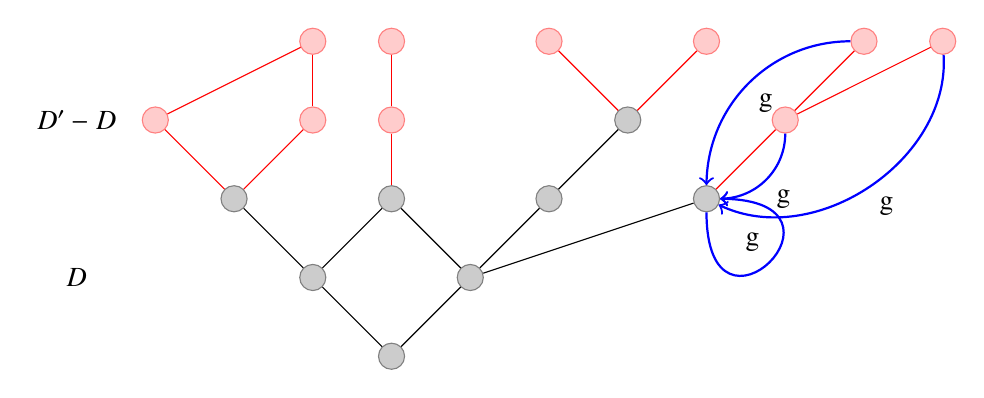
\begin{tikzpicture}
  [place/.style={circle,draw=black!50,fill=black!20},
  transition/.style={circle,draw=red!50,fill=red!20}]
  \node at (0, -2) [place] (p0) {};
  \node at (-1, -1) [place] (p1) {};
  \node at (1, -1) [place] (p2) {};
  \node at (-2, 0) [place] (p3) {};
  \node at (0, 0) [place] (p4) {};
  \node at (2, 0) [place] (p5) {};
  \node at (4, 0) [place] (p6) {};
  \node at (-3, 1) [transition] (p7) {};
  \node at (-1, 1) [transition] (p8) {};
  \node at (0, 1) [transition] (p9) {};
  \node at (3, 1) [place] (p10) {};
  \node at (5, 1) [transition] (p11) {};
  \node at (-1, 2) [transition] (p12) {};
  \node at (0, 2) [transition] (p13) {};
  \node at (2, 2) [transition] (p14) {};
  \node at (4, 2) [transition] (p15) {};
  \node at (6, 2) [transition] (p16) {};
  \node at (7, 2) [transition] (p17) {};
  \node at (-4,-1) {$D$};
  \node at (-4,1) {$D'-D$};
  \draw [-] (p0) to (p2);
  \draw [-] (p0) to (p1);
  \draw [-] (p1) to (p3);
  \draw [-] (p1) to (p4);
  \draw [-] (p2) to (p4);
  \draw [-] (p2) to (p5);
  \draw [-] (p2) to (p6);
  \draw [red,-] (p3) to (p7);
  \draw [red,-] (p3) to (p8);
  \draw [red,-] (p4) to (p9);
  \draw [-] (p5) to (p10);
  \draw [red,-] (p6) to (p11);
  \draw [red,-] (p7) to (p12);
  \draw [red,-] (p8) to (p12);
  \draw [red,-] (p9) to (p13);
  \draw [red,-] (p10) to (p14);
  \draw [red,-] (p10) to (p15);
  \draw [red,-] (p11) to (p16);
  \draw [red,-] (p11) to (p17);
  \draw [draw = blue, thick,-{Classical TikZ Rightarrow[length=1mm]}]
  (p6) edge [in=0, out=-90,looseness=20] node [auto] {g} (p6)
  (p11) edge [bend left=45] node [auto] {g} (p6)
  (p17) edge [bend left=60] node [auto] {g} (p6)
  (p16) edge [bend right=45] node [auto] {g} (p6);
\end{tikzpicture}
\textcolor{red}{newly added elements}

\textcolor{blue}{$g$ maps elements of $D'$  to their best underapproximations in $D$.}
\par}
What this means is that a morphism $f:D\rightarrow D'$ is really saying that $D'$ is larger than $D$.

6. A morphism $f:D\rightarrow D'$ in $Dom^{EP}$ is called \underline{embedding} and a corresponding $g:D'\rightarrow D$ is called \underline{projection}.
If you happen to take a course on program analysis, this pair of embedding $f$ and projection $g$ is closely related to the Galois connection theme.

Note that the definition doesn't say that there exists only one projection $g$ for a given embedding $f$. That is, there may be multiple projections. But this doesn't happend.
\begin{lemma}
  For every embedding $f:D\rightarrow D'$ and projections $g_1:D'\rightarrow D$ and $g_2:D'\rightarrow D$ for $f$, we have that $g_1 = g_2$.
\end{lemma}
\begin{proof}
  We will show that $g_1 \sqsubseteq g_2$. A similar argument can show the opposite inequality.
  \[g_1 = id_D \circ g_1 = (g_2 \circ f) \circ g_1 = g_2 (f \circ g_1) \sqsubseteq g_2 \circ id_{D'} = g_2\]
\end{proof}
We write $f^P$ to denote the unique projection for an embedding $f$.

7. The category $Dom^{EP}$ has an initial object, which is a singleton domain $(\{\bot\}, \sqsubseteq)$. It also has a co-limit for any $\omega$-chain. We will not prove this. But we point out one important property of these co-limits.

\begin{lemma}
  Consider the following co-cone of an $\omega$-chain $\Delta$:
  {\center
  \begin{tikzcd}
    \Delta = ( D_0 \arrow[r,"f_0"] \arrow[rrd,"h_0"] & D_1 \arrow[r,"f_1"] \arrow[rd,"h_1"] & D_2 \arrow[r,"f_2"] \arrow[d,"h_2"] & \ldots ) \\
    && D' &
  \end{tikzcd}
  \par}
  Let $h_i^P$ be the projection for the embedding $h_i$. Then, $D'$ is co-limiting\footnote{intuitively means least upper bound} iff \[\underline{\sqcup_{i=0}^\infty (h_i \circ h_i^P) = id_{D'}}\]
  (note that $h_i \circ h_i^P \sqsubseteq id_{D'}$ we can easily show that $\{h_i \circ h_i^P\}$ is an increasing chain in $[D'\rightarrow_C D']$. The underlined condition says that the least upper bound of the chain is $id$.)
\end{lemma}
This lemma says that \underline{the order on morphisms} plays an important role in deciding whether $D'$ is a co-limit or not. One important consequence is the following lemma.
\begin{lemma}
  A functor $F:Dom^{EP}\rightarrow Dom^{EP}$ is $\omega$-continuous if for every co-cone of an $\omega$-chain $\Delta$
  {\center
  \begin{tikzcd}
    D_0 \arrow[r,"f_0"] \arrow[rrd,"h_0"] & D_1 \arrow[r,"f_1"] \arrow[rd,"h_1"] & D_2 \arrow[r,"f_2"] \arrow[d,"h_2" ]& \cdots \\
    & & D' &
  \end{tikzcd}
  \par}
  $\sqcup_{i=0}^\infty h_i \circ h_i^P$ implies $\sqcup_{i=0}^\infty F(h_i) \circ F(h_i)^P = id_{F(D')}$
\end{lemma}
\begin{proof}
  This is a direct consequence of Lemma 2.
\end{proof}

8. Lemma 3 is our tool to check the $\omega$-continuity of a functor $F$ on $Dom^{EP}$. If this check passes, by the fixed point theorem, we know that there exists a domain D s.t. $F(D)\backsimeq D$.

(1) Our functor $F(\Omega) = (\Sigma + \Sigma + \mathbb{Z}\times \Omega + [\mathbb{Z}\rightarrow \Omega])_\bot$ is an example of such a functor.

(2) Another famous example is the following $G$ that defines the function space.
\[G(D) = [D\rightarrow_C D] \quad\cdots \quad \text{the domain of continuous functions in }D \]
For every $f:D\rightarrow D'$,
\begin{align*}
  &G(f):\underbrace{G(D)}_{[D\rightarrow_C D]}\rightarrow \underbrace{G(D')}_{[D'\rightarrow_C D']} \\
  &G(f)(h) = f \circ h \circ f^P \footnote{we are using the projection of $f$ here, if $f$ were just a continuous function, we couldn't do it}
\end{align*}
\underline{Exercise}
\begin{enumerate}
  \item Prove that $F$ and $G$ are indeed $\omega$-continuous.
  \item Prove Lemma 2. (This is not easy)
\end{enumerate}
If you are familar with program analysis and abstract interpretation, you might have noticed that there we de something similar when defining the abstract domain for function space. One thing to keep in mind is that in domain theory, $a\sqsubseteq b$ means that $b$ is more informative than $a$, while in program analysis $a\sqsubseteq b$ means that $a$ is more informative.
\end{document}
